\chapter{Separación}%
\label{cha:separacion}

\section{Concepto}%
\label{sec:concepto}
\begin{defi}
Un espacio $X$ es \textbf{Hausdorff} o $T_2$ si cada par de puntos distintos $x, y \in X$ existen entornos disjuntos:
\[
\exists V^x, V^y: V^x \cap V^y = \emptyset
\]
\end{defi}
Hay otras formas de separación, más débiles o más fuertes, pero nos contentaremos con ésta al ser la más intuitiva.

\begin{obs}
\begin{enumerate}
    \item Si existen entornos disjuntos, existen entornos abiertos disjuntos.
    \begin{demo}
        $\forall V^{\text{ent.}},\ \exists U^{\text{ent. ab.}}: V \supset U$
    \end{demo}
    \item Si $X$ es Hausdorff, los puntos son cerrados.
    \begin{demo}    
    Sea $x \in X$
    \[
    \forall y \in X \setminus \left\{ x \right\},\ \exists U^y \not\ni x \Rightarrow X \setminus \{x\} = \bigcup_{y \neq x} U^y  \text{ es abierto.} 
    \]
    También lo podemos ver como entorno de todos sus puntos.
    \end{demo}
    \item $\left( X, \mathcal{T}_{\text{CF}} \right)$ no es Hausdorff. Sin embargo, tiene puntos cerrados.
    \begin{demo}
        No es Hausdorff porque, si $X$ es infinito, dos abiertos cualesquiera se cortan.
        Sean $U_1, U_2 \in \mathcal{T}_{\text{CF}} \Rightarrow X \setminus U_1, X \setminus U_2$ son finitos y como $X$ es infinito $\Rightarrow \exists x \not\in X \setminus U_1 \cup X \setminus U_2 \Rightarrow x \in U_1 \cap U_2$.
    \end{demo}

    \item $\left( \mathbb{R}^n, \mathcal{T}_{u} \right)$ es Hausdorff. Como $\mathcal{T}_{u} \subset \mathcal{T}_{\text{rad}}$, esta última también es Hausdorff.
    \begin{demo}    
    Sean $x \neq y \Rightarrow B\left( x, \varepsilon \right) \cap B\left( y, \varepsilon \right) = \emptyset$ si $\varepsilon < \frac{\lVert x - y \rVert}{2}$.
    \end{demo}

    \item En $\left( X, \mathcal{T}_a \right)$ el punto $a$ no es cerrado. Por lo tanto no es Hausdorff. 
    \begin{demo}
    Veamos que $a$ no es cerrado: $a \not\in X \setminus \{a\} \Rightarrow X \setminus \{a\}$ no es abierto: $\forall x \neq a, U^x \supset \{a, x\} \ni a$.   
    \end{demo}
\end{enumerate}
\end{obs}

\begin{prop}
Sean $f, g: X \rightarrow Y$ continuas con $Y$ Hausdorff $\Rightarrow \{f = g\} = \{x \in X : f\left( x \right) = g\left( x \right)\}$ es cerrado.
\end{prop}
\begin{demo}
En primer lugar, veamos que si un punto cumple $f\left( x \right) \neq g\left( x \right) \Rightarrow$ tiene un entorno cuyos puntos cumplen todos que $f\left( y \right) \neq g\left( y \right)$. Con esto, tendremos que $\left\{ f \neq g \right\}$ es entorno de todos sus puntos y, por tanto, abierto.
\begin{enumerate}
    \item $f\left( x \right) \neq g\left( x \right) \xRightarrow{T_2} \exists V^{f\left( x \right)} \cap V^{g\left( x \right)} \stackrel{*}{=} \emptyset \xRightarrow{\text{cont.}} f^{-1}V^{f\left( x \right)} \cap g^{-1}V^{g\left( x \right)} = W^x$ entorno de $x$ (cada uno es entorno de $x$ y no son vacíos porque $x$ pertenece a ellos).

    \item Vemos que $W^x \cap \{f = g\} = \emptyset: y \in V^x \Rightarrow \begin{cases}
        f\left( y \right) \in V^{f\left( x \right)} \\
        g\left( y \right) \in V^{g\left( x \right)} 
    \end{cases} \xRightarrow{*} f\left( y \right) \neq g\left( y \right)$

    \item[1. + 2.] $X\setminus \{f = g\} = \{f \neq g\}$ es entorno de todos sus puntos, luego abierto, es decir, $\{f = g\}$ es cerrado.
\end{enumerate}
\end{demo}

\begin{coro}
Si $\left\{ f = g \right\}$ es un subconjunto denso, es decir, $\exists A \subset X: \overline{A} = X$ y $\left\{ f = g \right\}_A$, entonces $f \equiv g$.
\end{coro}
\begin{demo}
$f|_A = g|_A \Rightarrow \{f = g\} \supset A \xRightarrow{\text{prop.}} \overline{\left\{ f = g \right\}} = \{f = g\} \supset \overline{A} = X \Rightarrow \boxed{X = \left\{ f = g \right\}}$.
\end{demo}

\begin{obs}
Este último resultado nos permite extender de forma única una función continua $f$ a su adherencia.
\end{obs}

\begin{ej}[Importante]
Un caso importante en el que $Y$ es Hausdorff es: 
\[
f: X \rightarrow Y = \mathbb{R}
\]
\end{ej}

\begin{obs}
$f: X \rightarrow Y$ continua con $Y$ Hausdorff $\Rightarrow f^{-1}\left( y \right)$ cerrado $\forall y \in Y$.
\begin{demo}
Porque los puntos de $Y$ son cerrados y la preimagen de cerrados por continuidad es cerrada.
\end{demo}
\end{obs}

\section{Tabla de comportamiento}%
\label{sec:tabla_de_comportamiento}
Se trata de saber si la propiedad se conserva por las construcciones que hemos visto.

Se tiene que:
\begin{table}[H]
\centering
\begin{tabular}{| c | c | c | c | c |}
    \hline
    & Subespacios & Cocientes & Productos & Sumas\\
    \hline
    $T_2$ & $\Rightarrow$ & \ding{55} & $\Leftrightarrow$ & $\Leftrightarrow$\\
    \hline
\end{tabular}
\caption{\textit{Tabla que nos indica como se conserva la propiedad Hausdorff en distintas construcciones.}}
\end{table}
\begin{demo}
\begin{enumerate}
    \item\label{it:subespacio_hausdorff} Veamos como los subespacios conservan la propiedad: 

    Sea $Y \subset X = T_2: y_1, y_2 \in Y \Rightarrow \exists \underbrace{V^{y_1}}_{\text{En } X}  \cap \underbrace{V^{y_2}}_{\text{En } X} = \emptyset \Rightarrow \underbrace{\left( V^{y_1} \cap Y \right)}_{\text{En } Y}  \cap \underbrace{\left( V^{y_2} \cap Y \right)}_{\text{En } Y} = \emptyset$.

    \item Veamos un contraejemplo de un cociente que no conserva Hausdorff: 

    Sea $Y = \faktor{\mathbb{R}}{\mathbb{Q}}: \begin{rcases}
        y_1 = \mathbb{Q} \in Y\\
        y_2 = \sqrt{2} \in Y
    \end{rcases} \nexists V^{y_1} \cap V^{y_2} = \emptyset: $ todo entorno abierto de $\sqrt{2}$ contiene racionales, luego al saturar, contiene $\mathbb{Q}$. Con esto, todo abierto en el cociente (recordemos que en el cociente los abiertos son imágenes por proyección de los saturados) contiene este punto y, por tanto, la intersección nunca es disjunta.

    \item Veamos que el producto conserva la propiedad: 

    $X$ y $Y$ son ambos $T_2 \Leftrightarrow X \times Y$ Hausdorff.
    \begin{itemize}
        \item[$\Rightarrow)$] Tomamos $\left( x_1, y_1 \right) \neq \left( x_2, y_2 \right) \in X \times Y$. Esto es posible en dos casos:
        \begin{itemize}
            \item $x_1 \neq x_2$. Como $X$ es $T_2 \Rightarrow \exists V^{x_1} \cap V^{x_2} = \emptyset \Rightarrow \left( V^{x_1} \times Y \right) \cap \left( V^{x_2} \times Y \right) = \emptyset$ 
            \item $y_1 \neq y_2$ podemos hacer lo mismo porque $Y$ es también $T_2$.
        \end{itemize}

    %TODO: Corregir caption 
    \begin{figure}[H]
        \centering
        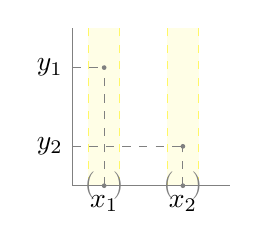
\begin{tikzpicture}
            \draw[-, gray] (0,0) -- (0,2);

            %Rectangulo izq
            \fill[fill=yellow!10, very thick, dashed] (0.2,2) rectangle (0.6,0);
            \draw[-, yellow!60] (0.2,0) -- (0.6,0);
            \draw[-, yellow!60, dashed] (0.2,0) -- (0.2,2);
            \draw[-, yellow!60, dashed] (0.6,0) -- (0.6,2);
            \fill[gray] (0.4,0) circle (0.03);

            %Rectangulo der
            \fill[fill=yellow!10, very thick, dashed] (1.2,2) rectangle (1.6,0);
            \draw[-, yellow!60] (1.2,0) -- (1.6,0);
            \draw[-, yellow!60, dashed] (1.2,0) -- (1.2,2);
            \draw[-, yellow!60, dashed] (1.6,0) -- (1.6,2);
            \fill[gray] (1.4,0) circle (0.03);

            \draw[-, gray] (0,0) -- (2,0) node[pos=0.11] {(}
                node[pos=0.29] {)}
                node[pos=0.61] {(}
                node[pos=0.79] {)};
            postaction={decorate}

            \node(x1) at (0.4,0) [below] {$x_1$};
            \node(x2) at (1.4,0) [below] {$x_2$};

            \fill[gray] (0.4,1.5) circle (0.03);
            \fill[gray] (1.4,0.5) circle (0.03);

            \node(y1) at (0,1.5) [left] {$y_1$};
            \node(y2) at (0,0.5) [left] {$y_2$};

            %Lineas 1
            \draw[-, gray, dashed] (x1) -- (0.4,1.5);
            \draw[-, gray, dashed] (y1) -- (0.4,1.5);

            %Lineas 2
            \draw[-, gray, dashed] (x2) -- (1.4,0.5);
            \draw[-, gray, dashed] (y2) -- (1.4,0.5);
        \end{tikzpicture}
        \captionsetup{font={color=gray}}
        \caption{\textit{Siendo $x_1 \neq x_2$ vemos que es posible separar los puntos $\left( x_1, y_1 \right)$ y $\left( x_2, y_2 \right)$ simplemente separando en el factor $X$ del producto.}}
    \end{figure}

    \item[$\Leftarrow)$] Sabemos que $X \approx X \times \left\{ y_0 \right\} \subset X \times Y$ que es $T_2 \xRightarrow{\ref{it:subespacio_hausdorff}.} X \times \left\{ y_0 \right\}$ es $T_2$ y, por homeomorfismo, $X$ también.
    \end{itemize} 

    \item Veamos que la suma conserva la propiedad:

    $X$ y $Y$ son ambos $T_2 \Leftrightarrow X + Y$ es Hausdorff.

    Único comentario: $x \in X$ e $y \in Y \Rightarrow X = V^x, Y = V^y$ y $X \cap Y = \emptyset$ (recordemos que hemos definido la suma como unión disjunta).

    Si $x$ e $y$ pertenecen ambos a $X$ ó a $Y$ simplemente aplicamos que son $T_2$.
\end{enumerate}    
\end{demo}
